%!TEX root=main.tex
\begin{section}{Dataset}
	\label{sec:dataset}
	The Broad Bioimage Benchmark Collection BBBC021 image set \cite{bbbc021} is a collection of 13,200 images from compound treatment on MCF-7 breast cancer cells. Each image consists of three channels: the cells are labeled for DNA, F-actin, and B-tubulin and imaged with fluorescence microscopy. Metadata on compound treatment and concentration is also available\cite{Caie1913}. In all, 113 compounds have been used, each with varying concentrations and tested between 2 and 3 times each. Mechanism of action (MoA) labels are available for 103 compound-concentrations (38 compounds tested at between one and seven different concentrations each). In all, 13 MoAs (including the neutral control, DMSO) were available: 6 of the 12 MoAs were assigned visually.  DMSO treatments were treated as neutral control and assigned a separate label. The others were defined based on information on the respective compounds in the available literature.  We choose 1684 images from the BBBC021 dataset that are representative of all of the MoAs present. The distribution of the images according to MoA classes is shown in \autoref{fig:classdistribution}. The images are preprocessed and normalized as described in \cite{Godinez2017}. From the 1684 images, we create two datasets with different augmentation strategies:

		\begin{figure}[t]
			\centering
			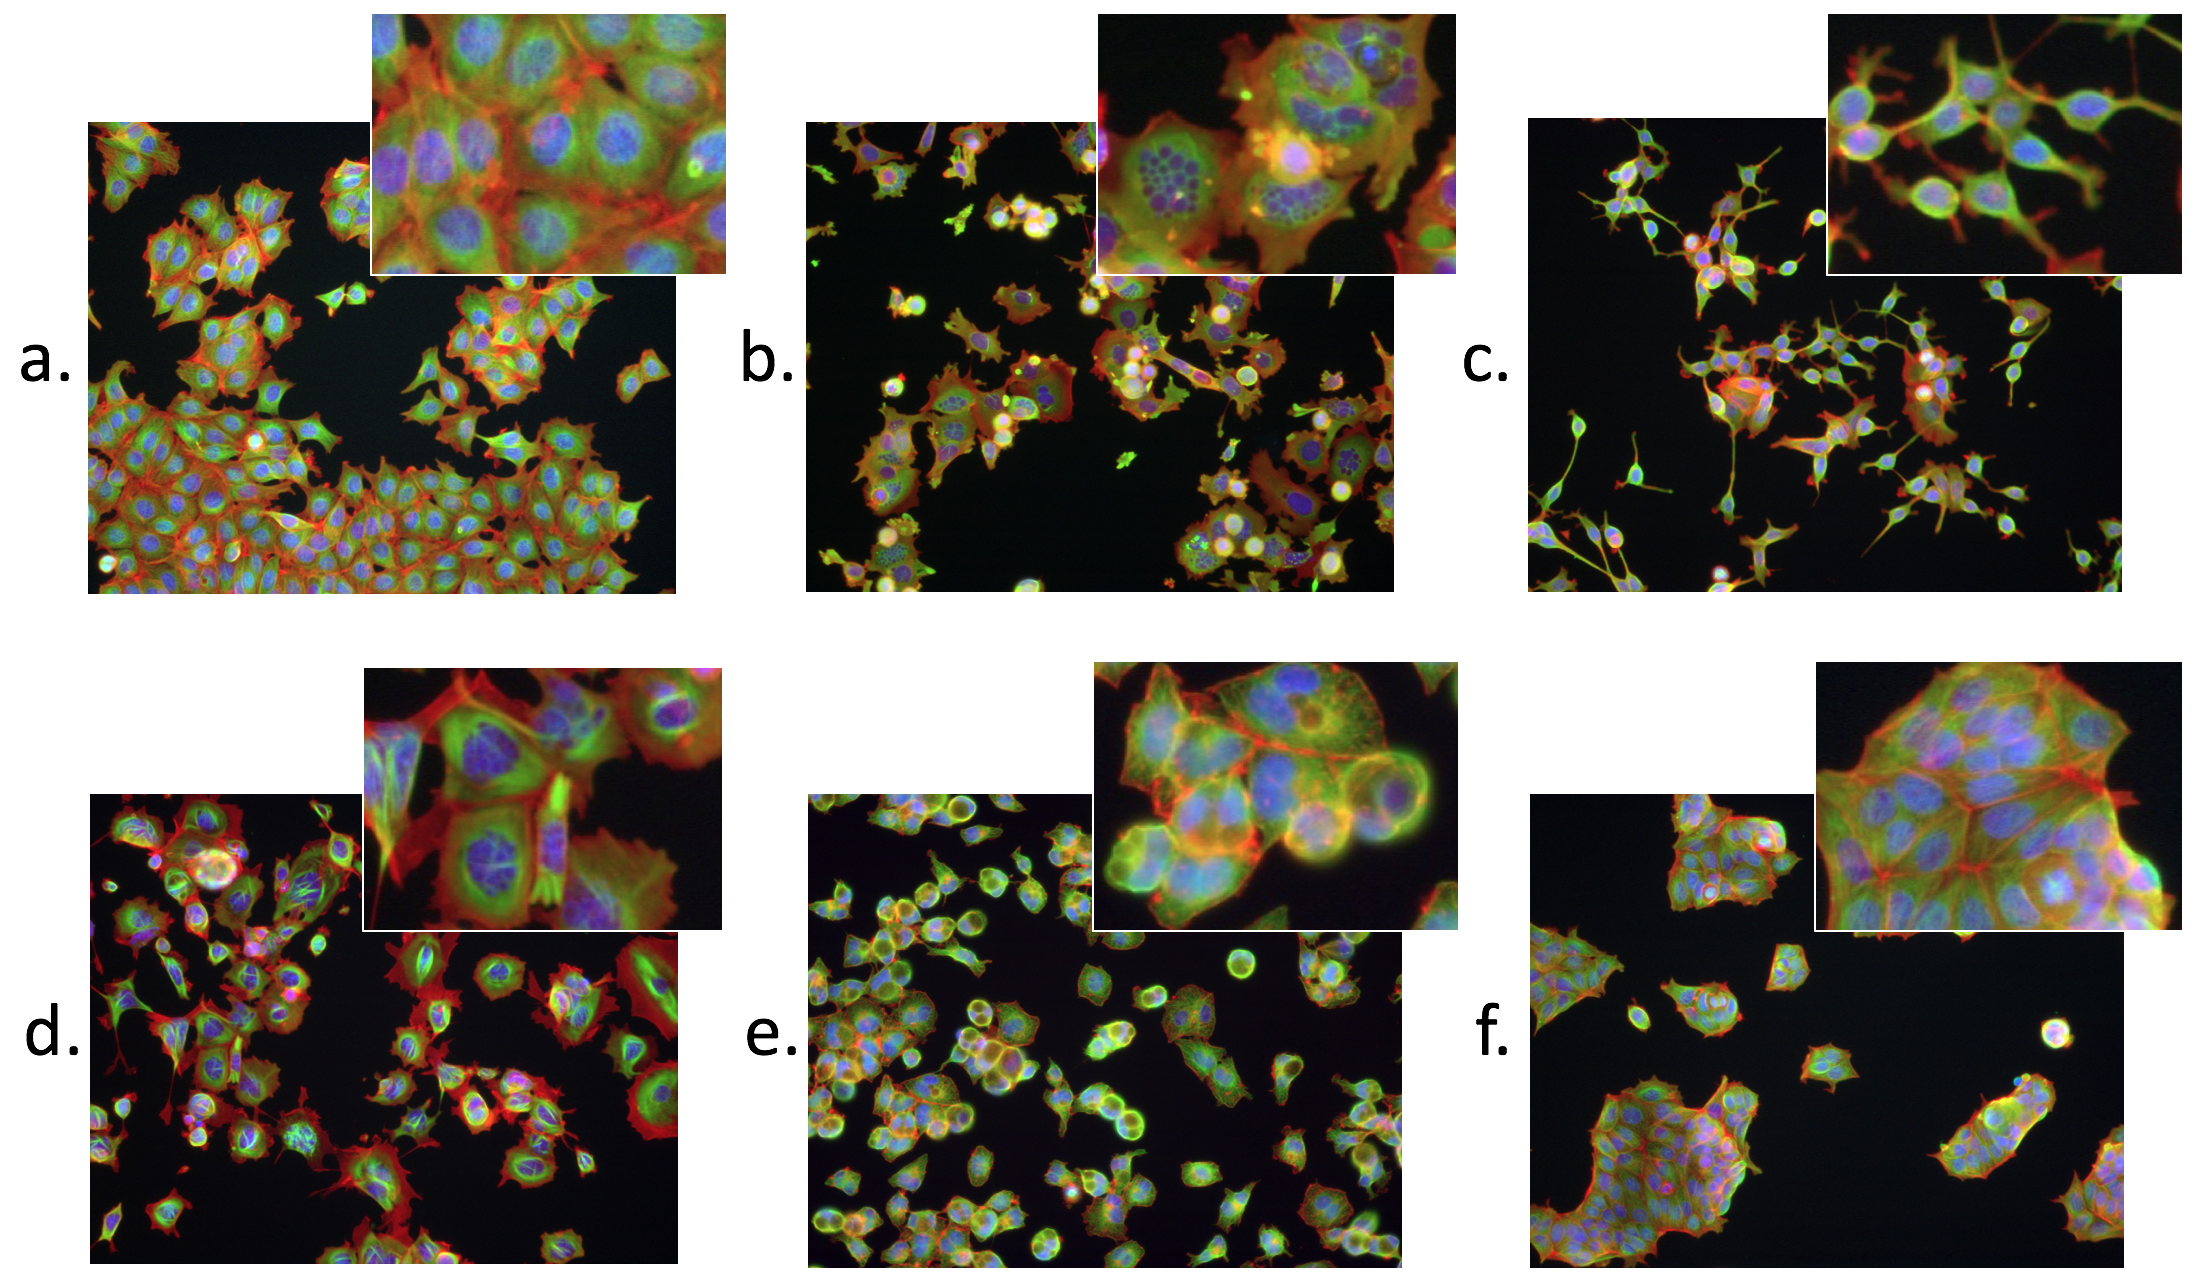
\includegraphics[width=4.75in]{bbbc021_moa_examples_w_insets.png}
			\caption{\textsf{Example images from the BBBC021\cite{bbbc021} dataset showing phenotypes from treatment with compound-concentration pairs with different mechanisms of action: a) DSMO (neutral control), b) Microtubule destabilizer, c) Cholesterol lowering, d) Microtubule stabilizer,  e) Actin disrupter, f) Epithelial. DNA staining is shown in blue, the F-actin staining in red and the Β-tubulin staining in green. The insets show a magnified view of the same phenotypes.}}
			\label{fig:bbbc_whole}
	\end{figure}
	
	\begin{itemize}
		\item \textit{Dataset A}: Images in this dataset are 1024x1280 pixesl wide with 3 channels. They are augmented to produce five copies as
		\begin{enumerate*}
			\item $90^{\circ}$ rotation,
			\item a horizontal mirror,
			\item vertical mirror,
			\item $90^{\circ}$ rotation of horizontal mirror and
			\item $90^{\circ}$ rotation of vertical mirror
		\end{enumerate*}. Total number of images in the dataset is $1684*6$ (five rotations + original) $= 10104$. We take a 90-10 split and create a training set of 9093 images and validation set of 1011 images. The total size of the images on disk are 38GB. 
		\item
		\textit{Dataset B}: This is a larger dataset. The dimensions of the images in this dataset are 724x724 pixesl with 3 channels. Similar to Dataset A, all images have 5 additional augmentations. Additionally, each image is rotated by $15^{\circ}$ to create 23 more augmentations. The total size of the images on disk are  512GB. Among them, 313282 images are used for training and 35306 are used for validation. \\\\
\noindent Ideally, we would have allocated a representative out-of-sample set of images as a validation set. However due to the paucity of MOA annotations in this dataset, and the fact that the main objective of this exercise is to reduce time to convergence, we allow for the fact that the validation dataset may contain an augmented version of an image in the training data, although never a copy of the same image. 
	\end{itemize}
	\begin{figure}[h]
	  \centering	
	    %\includegraphics[width=\textwidth]
	    \includegraphics[width=3.5in]
	    {wgrid_figure2.png}
	  \caption{Class distribution for the 1684 training images used in our experiment.}
	  \label{fig:classdistribution}
	\end{figure}
%	\begin{subsection}{Shuffling input data}
%		\label{sec:shuffling}
%		Parallel workers are more effective when there is variation between the batches. Hence, we shuffle the image order for each worker. Similar variations between epochs also helps in faster convergence. To ensure this, we use two rounds of random shuffling. First, slices are created following the frequency distribution of the classes. For example, if the slice size is 256, $\frac{440}{1684}*256=67$ images are picked from class 12, $\frac{168}{1684}*256=26$ images are picked from class 8 and so on. Data in each slice are then randomly shuffled as follows:\\
%% # Frequency distribution of images taken
%% # Fig. 2
%% freq_dist_source = [60, 144, 72, 108, 96, 144, 88, 40, 168, 144, 84, 96, 440]
%\begin{tcolorbox}
%		\begin{verbatim}
%Loop:
%    unread_images = sum(x for x in freq_dist_source)
%
%    # Choose number of imagers per slice
%    slice_size_per_class = [min(int(x*slice_size/unread_images)
%                           , x) for x in freq_dist_source]
%
%    # Remove picked images from list of input images
%    freq_dist_source = np.asarray(freq_dist_source) - 
%                       np.asarray(slice_size_per_class)
%		\end{verbatim} 
%	\end{tcolorbox}
%			%\begin{lstlisting}
%			%# Frequency distribution of images taken
%			%# Fig. 2
%			%freq_dist_source = [60, 144, 72, 108, 96, 144, 88, 40, 168, 144, 84, 96, 440]
%	        %
%			%Loop:
%			%	unread_images = sum(x for x in freq_dist_source)
%	        %
%			%	# Choose number of imagers per slice
%			%	slice_size_per_class = [min(int(x*slice_size/unread_images), x) for x in freq_dist_source]
%	        %
%			%	# Remove picked images from list of input images
%			%	freq_dist_source = np.asarray(freq_dist_source) - np.asarray(slice_size_per_class)
%			%\end{lstlisting}	
%
%\noindent Finally, during ingestion, each worker reads data into buffers and shuffles them to produce batches. This is achieved by the Dataset API in TensorFlow \cite{TFDataset} as shown below. The random number generator in each worker is seeded with its unique identifier.
%	\begin{tcolorbox}
%			\begin{verbatim}
%# Read all slices in parallel into an interleaved buffer 
%#  using 4 threads, 8 images at a time.
%dataset = dataset.apply(
%    tf.contrib.data.parallel_interleave(
%        tf.data.TFRecordDataset(
%            filename, buffer_size=buffer_size),
%        cycle_length=4,
%        block_length=8,
%        sloppy=True
%        )
%    )
%
%# Shuffle the images in the buffer
%dataset = dataset.shuffle()                  	
%			\end{verbatim}
%	\end{tcolorbox}
%		% \end{itemize}
%	\end{subsection}
\end{section}





